\documentclass[conference,10pt]{IEEEtran}
\IEEEoverridecommandlockouts
\usepackage{cite}
\usepackage{amsmath,amssymb}
\usepackage{graphicx}
\usepackage{booktabs}
\usepackage{multirow}
\usepackage{xcolor}
\usepackage{tikz}
\usetikzlibrary{positioning,arrows.meta,calc}
\usepackage[hidelinks]{hyperref}
\usepackage{url}
\makeatletter\g@addto@macro\UrlBreaks{\UrlOrds}\makeatother
\graphicspath{{../outputs/figures/}}

\newcommand{\NHWTest}{228}
\newcommand{\NSevTest}{2}
\newcommand{\HotRateTest}{11.5\%}
\newcommand{\NSeries}{43}
\newcommand{\NTestPairs}{220{,}332}
\newcommand{\NTestForecasts}{31{,}476}
\newcommand{\BestFM}{Chronos-2+cov}
\newcommand{\CRPSbestFM}{0.988}
\newcommand{\BestBaseline}{Quantile-LSTM}
\newcommand{\CRPSbaseline}{0.935}
\newcommand{\CRPSChronostwocov}{0.988}
\newcommand{\CRPSSChronostwocov}{0.173}
\newcommand{\MAEChronostwocov}{1.38}
\newcommand{\CovChronostwocov}{0.75}
\newcommand{\CRPSChronostwocovLone}{0.616}
\newcommand{\CRPSChronostwocovLthree}{0.967}
\newcommand{\CRPSChronostwocovLseven}{1.179}
\newcommand{\CRPSChronostwo}{0.989}
\newcommand{\CRPSSChronostwo}{0.172}
\newcommand{\MAEChronostwo}{1.38}
\newcommand{\CovChronostwo}{0.77}
\newcommand{\CRPSChronostwoLone}{0.614}
\newcommand{\CRPSChronostwoLthree}{0.962}
\newcommand{\CRPSChronostwoLseven}{1.197}
\newcommand{\CRPSChronosBolt}{1.019}
\newcommand{\CRPSSChronosBolt}{0.147}
\newcommand{\MAEChronosBolt}{1.42}
\newcommand{\CovChronosBolt}{0.78}
\newcommand{\CRPSChronosBoltLone}{0.603}
\newcommand{\CRPSChronosBoltLthree}{0.974}
\newcommand{\CRPSChronosBoltLseven}{1.274}
\newcommand{\CRPSQuantileLSTM}{0.935}
\newcommand{\CRPSSQuantileLSTM}{0.217}
\newcommand{\MAEQuantileLSTM}{1.30}
\newcommand{\CovQuantileLSTM}{0.78}
\newcommand{\CRPSQuantileLSTMLone}{0.606}
\newcommand{\CRPSQuantileLSTMLthree}{0.921}
\newcommand{\CRPSQuantileLSTMLseven}{1.099}
\newcommand{\CRPSARanomaly}{0.943}
\newcommand{\CRPSSARanomaly}{0.211}
\newcommand{\MAEARanomaly}{1.31}
\newcommand{\CovARanomaly}{0.82}
\newcommand{\CRPSARanomalyLone}{0.593}
\newcommand{\CRPSARanomalyLthree}{0.932}
\newcommand{\CRPSARanomalyLseven}{1.112}
\newcommand{\CRPSPersistence}{1.063}
\newcommand{\CRPSSPersistence}{0.110}
\newcommand{\MAEPersistence}{1.47}
\newcommand{\CovPersistence}{0.80}
\newcommand{\CRPSPersistenceLone}{0.602}
\newcommand{\CRPSPersistenceLthree}{1.020}
\newcommand{\CRPSPersistenceLseven}{1.325}
\newcommand{\CRPSClimatology}{1.194}
\newcommand{\CRPSSClimatology}{0.000}
\newcommand{\MAEClimatology}{1.69}
\newcommand{\CovClimatology}{0.77}
\newcommand{\CRPSClimatologyLone}{1.188}
\newcommand{\CRPSClimatologyLthree}{1.193}
\newcommand{\CRPSClimatologyLseven}{1.197}
\newcommand{\ValCRPSChronostwocov}{0.930}
\newcommand{\ValCRPSChronostwo}{0.995}
\newcommand{\ValCRPSChronosBolt}{1.071}
\newcommand{\ValCRPSQuantileLSTM}{0.897}
\newcommand{\ValCRPSARanomaly}{0.946}
\newcommand{\ValCRPSPersistence}{1.113}
\newcommand{\ValCRPSClimatology}{1.085}
\newcommand{\CovBetterYears}{4}
\newcommand{\CovYearsTotal}{6}
\newcommand{\CRPSChronostwocovYtwozeroonenine}{0.932}
\newcommand{\CRPSChronostwoYtwozeroonenine}{0.904}
\newcommand{\CRPSChronostwocovYtwozerotwozero}{0.958}
\newcommand{\CRPSChronostwoYtwozerotwozero}{0.996}
\newcommand{\CRPSChronostwocovYtwozerotwoone}{0.871}
\newcommand{\CRPSChronostwoYtwozerotwoone}{0.885}
\newcommand{\CRPSChronostwocovYtwozerotwotwo}{0.911}
\newcommand{\CRPSChronostwoYtwozerotwotwo}{0.943}
\newcommand{\CRPSChronostwocovYtwozerotwothree}{1.317}
\newcommand{\CRPSChronostwoYtwozerotwothree}{1.203}
\newcommand{\CRPSChronostwocovYtwozerotwofour}{0.937}
\newcommand{\CRPSChronostwoYtwozerotwofour}{1.005}
\newcommand{\BSShotChronostwocov}{0.285}
\newcommand{\BSShwChronostwocov}{0.112}
\newcommand{\AUChwChronostwocov}{0.964}
\newcommand{\AUChotChronostwocov}{0.888}
\newcommand{\BSShotChronostwo}{0.281}
\newcommand{\BSShwChronostwo}{0.079}
\newcommand{\AUChwChronostwo}{0.974}
\newcommand{\AUChotChronostwo}{0.886}
\newcommand{\BSShotChronosBolt}{0.280}
\newcommand{\BSShwChronosBolt}{-0.208}
\newcommand{\AUChwChronosBolt}{0.982}
\newcommand{\AUChotChronosBolt}{0.895}
\newcommand{\BSShotQuantileLSTM}{0.344}
\newcommand{\BSShwQuantileLSTM}{0.183}
\newcommand{\AUChwQuantileLSTM}{0.983}
\newcommand{\AUChotQuantileLSTM}{0.910}
\newcommand{\BSShotARanomaly}{0.297}
\newcommand{\BSShwARanomaly}{0.142}
\newcommand{\AUChwARanomaly}{0.976}
\newcommand{\AUChotARanomaly}{0.903}
\newcommand{\BSShotPersistence}{0.277}
\newcommand{\BSShwPersistence}{-0.416}
\newcommand{\AUChwPersistence}{0.982}
\newcommand{\AUChotPersistence}{0.912}
\newcommand{\BSShotClimatology}{0.000}
\newcommand{\BSShwClimatology}{0.000}
\newcommand{\AUChwClimatology}{0.908}
\newcommand{\AUChotClimatology}{0.565}
\newcommand{\FocusCRPSChronostwocov}{0.921}
\newcommand{\FocusCRPSChronostwocovRH}{0.907}
\newcommand{\FocusCRPSChronostwo}{0.921}
\newcommand{\FocusCRPSChronosBolt}{0.957}
\newcommand{\FocusCRPSChronosTfive}{1.016}
\newcommand{\FocusCRPSQuantileLSTM}{0.879}
\newcommand{\FocusCRPSARanomaly}{0.888}
\newcommand{\FocusCRPSPersistence}{1.007}
\newcommand{\FocusCRPSClimatology}{1.116}
\newcommand{\CSIorangeChronostwocov}{0.15}
\newcommand{\CSIyellowChronostwocov}{0.38}
\newcommand{\PODorangeChronostwocov}{0.20}
\newcommand{\FARorangeChronostwocov}{0.60}
\newcommand{\CSIorangeChronostwocovRH}{0.21}
\newcommand{\CSIyellowChronostwocovRH}{0.39}
\newcommand{\PODorangeChronostwocovRH}{0.32}
\newcommand{\FARorangeChronostwocovRH}{0.64}
\newcommand{\CSIorangeChronostwo}{0.27}
\newcommand{\CSIyellowChronostwo}{0.39}
\newcommand{\PODorangeChronostwo}{0.66}
\newcommand{\FARorangeChronostwo}{0.68}
\newcommand{\CSIorangeChronosBolt}{0.30}
\newcommand{\CSIyellowChronosBolt}{0.40}
\newcommand{\PODorangeChronosBolt}{0.69}
\newcommand{\FARorangeChronosBolt}{0.65}
\newcommand{\CSIorangeChronosTfive}{0.30}
\newcommand{\CSIyellowChronosTfive}{0.36}
\newcommand{\PODorangeChronosTfive}{0.71}
\newcommand{\FARorangeChronosTfive}{0.66}
\newcommand{\CSIorangeQuantileLSTM}{0.20}
\newcommand{\CSIyellowQuantileLSTM}{0.40}
\newcommand{\PODorangeQuantileLSTM}{0.27}
\newcommand{\FARorangeQuantileLSTM}{0.57}
\newcommand{\CSIorangeARanomaly}{0.26}
\newcommand{\CSIyellowARanomaly}{0.40}
\newcommand{\PODorangeARanomaly}{0.46}
\newcommand{\FARorangeARanomaly}{0.62}
\newcommand{\CSIorangePersistence}{0.27}
\newcommand{\CSIyellowPersistence}{0.41}
\newcommand{\PODorangePersistence}{0.36}
\newcommand{\FARorangePersistence}{0.49}
\newcommand{\CSIorangeClimatology}{0.04}
\newcommand{\CSIyellowClimatology}{0.16}
\newcommand{\PODorangeClimatology}{0.11}
\newcommand{\FARorangeClimatology}{0.94}
\newcommand{\AllCSIorangeChronostwocov}{0.13}
\newcommand{\AllCSIyellowChronostwocov}{0.35}
\newcommand{\AllCSIorangeChronostwocovRH}{0.21}
\newcommand{\AllCSIyellowChronostwocovRH}{0.39}
\newcommand{\AllCSIorangeChronostwo}{0.20}
\newcommand{\AllCSIyellowChronostwo}{0.37}
\newcommand{\AllCSIorangeChronosBolt}{0.23}
\newcommand{\AllCSIyellowChronosBolt}{0.38}
\newcommand{\AllCSIorangeChronosTfive}{0.30}
\newcommand{\AllCSIyellowChronosTfive}{0.36}
\newcommand{\AllCSIorangeQuantileLSTM}{0.16}
\newcommand{\AllCSIyellowQuantileLSTM}{0.40}
\newcommand{\AllCSIorangeARanomaly}{0.21}
\newcommand{\AllCSIyellowARanomaly}{0.39}
\newcommand{\AllCSIorangePersistence}{0.19}
\newcommand{\AllCSIyellowPersistence}{0.40}
\newcommand{\AllCSIorangeClimatology}{0.04}
\newcommand{\AllCSIyellowClimatology}{0.12}
\newcommand{\NSevPairs}{6}
\newcommand{\BootFM}{Chronos-2+cov}
\newcommand{\BootBL}{Quantile-LSTM}
\newcommand{\BootCRPS}{0.053}
\newcommand{\BootCRPSlo}{0.044}
\newcommand{\BootCRPShi}{0.061}
\newcommand{\BootBrierhw}{0.0005}
\newcommand{\BootBrierhwlo}{0.0003}
\newcommand{\BootBrierhwhi}{0.0008}
\newcommand{\BootBrierpninezero}{0.0066}
\newcommand{\BootBrierpninezerolo}{0.0052}
\newcommand{\BootBrierpninezerohi}{0.0080}
\newcommand{\BootCRPSleadone}{0.011}
\newcommand{\BootCRPSleadonelo}{0.006}
\newcommand{\BootCRPSleadonehi}{0.016}
\newcommand{\BootCRPSleadthree}{0.046}
\newcommand{\BootCRPSleadthreelo}{0.040}
\newcommand{\BootCRPSleadthreehi}{0.052}
\newcommand{\BootCRPSleadseven}{0.080}
\newcommand{\BootCRPSleadsevenlo}{0.066}
\newcommand{\BootCRPSleadsevenhi}{0.095}
\newcommand{\LocMAEraw}{2.00}
\newcommand{\LocMAEcor}{1.45}
\newcommand{\LocCRPSraw}{1.53}
\newcommand{\LocCRPScor}{1.03}
\newcommand{\LocPointHW}{129}
\newcommand{\HumidMumbai}{360}
\newcommand{\TmaxhwMumbai}{34}
\newcommand{\HumidRecentMumbai}{136}
\newcommand{\HumidPerYearMumbai}{10.6}
\newcommand{\HImaxMumbai}{44.7}
\newcommand{\IMDOrangeMumbai}{0}
\newcommand{\HumidRatnagiri}{153}
\newcommand{\TmaxhwRatnagiri}{12}
\newcommand{\HumidRecentRatnagiri}{66}
\newcommand{\HumidPerYearRatnagiri}{4.5}
\newcommand{\HImaxRatnagiri}{44.0}
\newcommand{\IMDOrangeRatnagiri}{0}
\newcommand{\HumidPune}{14}
\newcommand{\TmaxhwPune}{11}
\newcommand{\HumidRecentPune}{3}
\newcommand{\HumidPerYearPune}{0.4}
\newcommand{\HImaxPune}{41.7}
\newcommand{\IMDOrangePune}{0}
\newcommand{\TFiveCorr}{0.997}
\newcommand{\TFiveBSsamp}{0.0913}
\newcommand{\TFiveBSquant}{0.0912}
\newcommand{\FTsteps}{300}
\newcommand{\FTminutes}{430}
\newcommand{\TFiveSamples}{20}
\newcommand{\SpeedPersistence}{$>$1000}
\newcommand{\SpeedClimatology}{$>$1000}
\newcommand{\SpeedChronostwocov}{10}
\newcommand{\SpeedARanomaly}{18930}
\newcommand{\SpeedChronosTfive}{3}
\newcommand{\SpeedChronostwo}{97}
\newcommand{\SpeedChronosBolt}{389}
\newcommand{\SpeedQuantileLSTM}{44688}
\newcommand{\SpeedChronostwocovRH}{5}

% shrink a table to the line width only when it is wider
\newsavebox{\fitboxbin}
\newcommand{\fitbox}[1]{\sbox{\fitboxbin}{#1}\ifdim\wd\fitboxbin>\linewidth\resizebox{\linewidth}{!}{\usebox{\fitboxbin}}\else\usebox{\fitboxbin}\fi}

\begin{document}

\title{HeatCast-FM: Probabilistic Heatwave Early Warning for Mumbai-Pune using Generative Time-Series Foundation Models}

\author{\IEEEauthorblockN{Aditya Ravi}
\IEEEauthorblockA{Department of Information Technology (AI \& DS)\\
K. J. Somaiya College of Engineering, Mumbai\\
Roll No. 16014223004\\
aditya.ravi@somaiya.edu}
\and
\IEEEauthorblockN{Dirshak Deep Patro}
\IEEEauthorblockA{Department of Information Technology (AI \& DS)\\
K. J. Somaiya College of Engineering, Mumbai\\
Roll No. 16014223033\\
dirshak.p@somaiya.edu}}

\IEEEaftertitletext{\vspace{-0.6\baselineskip}\begin{center}\small Code and data: \url{https://github.com/aditya-ravi11/HeatCastFM}\\ Live demo: \url{https://aditya-ravi11.github.io/HeatCastFM/}\end{center}\vspace{0.2\baselineskip}}
\maketitle

{\small\bfseries\noindent\textit{Abstract:}\ IMD issues heatwave warnings with station rules. Plains stations need Tmax of at least 40\,\textdegree C and a departure of at least 4.5\,\textdegree C from normal. Coastal stations need at least 37\,\textdegree C. We test whether pretrained time-series foundation models, used without any training on Indian data, can serve as the forecasting core of a region-specific warning system for the IMD Mumbai-Pune region.

HeatCast-FM runs Chronos, Chronos-Bolt and Chronos-2 on IMD 1\textdegree{} gridded Tmax for 7 Maharashtra cities and 36 inland cells. It issues a 7-day forecast every day of March-June and converts each one into probabilities of a hot day (Tmax above its local 90th percentile), an IMD heatwave and a severe heatwave, and then into Green-to-Red warnings. We compare these models with persistence, climatology, an autoregressive model and a quantile LSTM trained on 1951-2014.

Over \NTestForecasts{} test forecasts from 2019-2024, Chronos-2 with covariates reached a CRPS of \CRPSChronostwocov\,\textdegree C, against \CRPSClimatology{} for climatology and \CRPSPersistence{} for persistence. The trained LSTM remained best at \CRPSQuantileLSTM\,\textdegree C. The gap between them was small at a 1-day lead and grew with lead time. All models separated heatwave days well (AUC 0.96-0.98). Chronos intervals were too narrow.

A point correction against city-level data, which stands in for IoT weather stations, roughly halved the error at the coast. At Mumbai the heat index passed the NOAA Danger level on \HumidMumbai{} March-June days in 1991-2024 that the Tmax rule did not flag, against \TmaxhwMumbai{} Tmax-rule heatwave days.
\par}\smallskip

{\small\bfseries\noindent\textit{Index Terms:}\ heatwave, early warning, time-series foundation model, Chronos, probabilistic forecasting, IMD, Maharashtra
\par}\medskip

\section{Introduction}
Heatwaves in India have grown longer and more frequent over the central and northwestern parts of the country \cite{rohini2016heat,pai2013heat}. They reduce labour capacity, raise hospital admissions and stress power and water supply. IMD issues district-level heatwave warnings using station criteria \cite{imdfaq}. The criteria differ for plains, coastal and hill stations, so a single temperature does not mean the same thing everywhere. For example, 38\,\textdegree C in early March can meet the heatwave rule in Mumbai, while in May it is an ordinary afternoon in Nagpur.

The use case KJS-CES-01 asks for region-wise maximum temperature forecasts, heatwave prediction and severity classification, and validation against ground observations. Recent work in India has trained machine learning models for this task station by station or city by city \cite{ratnam2023ml,khan2022hybrid,choudary2025compare}. These models need long training records, retraining for each new location, and care to avoid overfitting to a few extreme seasons.

Time-series foundation models offer a different route. Chronos \cite{ansari2024chronos} scales and quantizes a series into tokens and trains a T5 language model \cite{raffel2020t5} on them. It then generates future values by sampling tokens, which gives a set of possible futures rather than one number. Chronos-Bolt emits quantiles directly. Chronos-2 \cite{ansari2025chronos2} adds group attention so that covariates and related series can inform the forecast. All three are used here zero-shot: they see the recent temperature history at forecast time and are never trained on Indian data.

This work makes four contributions:
\begin{enumerate}
\item A rolling-origin benchmark of three Chronos models against four trained or statistical baselines on \NSeries{} Maharashtra series for the March-June seasons of 2015-2024.
\item A conversion from quantile forecasts to IMD rule probabilities that handles plains and coastal criteria in one formula. We also give a colour warning scheme tuned on held-out years.
\item A point validation step (Objective 3 of the use case). It compares grid forecasts with city-point data and ships a loader for real AWS files.
\item An analysis of humid heat at the Konkan coast that the Tmax-only rule misses.
\end{enumerate}

\section{Related Work}
\textbf{Heatwave climatology in India.} Pai et al. \cite{pai2013heat} built a 50-year station climatology of heatwaves and found rising frequency over much of the country. Rohini et al. \cite{rohini2016heat} used IMD gridded temperature \cite{srivastava2009grid} with a 90th percentile definition and linked heatwave variability to Indian Ocean and Pacific sea surface temperatures. We use the same gridded product and a 90th percentile hot-day event alongside the IMD rule.

\textbf{Machine learning forecasts.} Ratnam et al. \cite{ratnam2023ml} compared ten machine learning regressors for 10-day Tmax anomaly forecasts over India in March-June. Khan and Maity \cite{khan2022hybrid} combined convolutional and LSTM layers for multi-step Tmax prediction in 28 Indian cities. Choudary et al. \cite{choudary2025compare} compared tree ensembles, CNNs, LSTMs and Transformers for heatwave prediction in Tamil Nadu and found tree ensembles strong at short range. All of these train on the target region.

\textbf{Time-series foundation models.} TimesFM \cite{das2024timesfm} is a decoder-only model trained on about 100 billion time points. Moirai \cite{woo2024moirai} is a masked encoder trained on 27 billion observations. Chronos \cite{ansari2024chronos} and Chronos-2 \cite{ansari2025chronos2} come from Amazon. We did not find published work that tests these models on Indian heatwave forecasting, which is the gap this project addresses.

\textbf{Verification.} We score probabilistic forecasts with the continuous ranked probability score (CRPS), a strictly proper score \cite{gneiting2007scoring}, and event probabilities with the Brier score \cite{brier1950}.

\section{Study Area and Data}
\subsection{Regions}
Table~\ref{tab:regions} lists the seven focus regions. Mumbai and Ratnagiri use the IMD coastal rule, and the rest use the plains rule. For each city we take the nearest IMD 1\textdegree{} cell with at least 95\% valid days. To obtain enough events for verification we also include all 36 inland cells between 16.5-21.5\textdegree N and 74.5-79.5\textdegree E. These cover interior Maharashtra and small parts of the neighbouring states. In total there are \NSeries{} series.

\begin{table*}[t]
\centering
\caption{Focus regions, their IMD grid cells, mean May normal Tmax (1981-2010) and event days in the March-June test seasons 2019-2024.}
\label{tab:regions}
\footnotesize
\setlength{\tabcolsep}{4pt}
\fitbox{%
\begin{tabular}{lllllrrrr}
\toprule
Region & Zone & Rule & City (N, E) & Cell (N, E) & May $N$ & Hot & HW & Sev \\
\midrule
Mumbai & Konkan & coastal & 19.08, 72.88 & 19.5, 72.5 & 35.8 & 98 & 0 & 0 \\
Ratnagiri & Konkan & coastal & 16.99, 73.31 & 16.5, 73.5 & 34.1 & 170 & 0 & 0 \\
Pune & Madhya Maharashtra & plains & 18.52, 73.86 & 18.5, 73.5 & 34.9 & 162 & 0 & 0 \\
Jalgaon & Madhya Maharashtra & plains & 21.00, 75.56 & 21.5, 75.5 & 40.4 & 76 & 7 & 0 \\
Sambhajinagar & Marathwada & plains & 19.88, 75.34 & 19.5, 75.5 & 39.9 & 95 & 5 & 0 \\
Nagpur & Vidarbha & plains & 21.15, 79.09 & 21.5, 79.5 & 40.5 & 92 & 9 & 1 \\
Chandrapur & Vidarbha & plains & 19.96, 79.30 & 19.5, 79.5 & 41.9 & 52 & 14 & 0 \\
36 box cells & Interior & plains & -- & 16.5-21.5N, 74.5-79.5E & -- & 2888 & 193 & 1 \\
\bottomrule
\end{tabular}}
\end{table*}


\subsection{Data sources}
\textbf{IMD gridded temperature.} Daily Tmax and Tmin on a 1\textdegree{} grid for 1951-2024 were downloaded with IMDLIB \cite{nandi2024imdlib}. The grid is built from about 395 quality-controlled stations using Shepard's angular distance weighting \cite{srivastava2009grid}.

\textbf{Station proxy.} The project has no AWS readings yet. As a stand-in we use daily Tmax, Tmin, mean and minimum relative humidity for 1990-2024 at the exact city coordinates from the Open-Meteo archive \cite{zippenfenig2024openmeteo}, which is based on ERA5 reanalysis \cite{hersbach2020era5}. A loader for real AWS files (timestamp, temperature, humidity) applies range and step checks, drops days with less than 75\% coverage and writes the same daily fields. Real stations can therefore replace the proxy without code changes.

\subsection{Event definitions}
Normals are the 1981-2010 day-of-year mean, smoothed with a 31-day circular window. This period keeps all validation and test years out of the baseline. Because departure equals Tmax minus normal, each IMD rule reduces to a single Tmax threshold for each day:
\begin{align}
\theta^{\text{HW}}_{\text{plains}} &= \min\{\max(40,\ N+4.5),\ 45\},\\
\theta^{\text{SEV}}_{\text{plains}} &= \min\{\max(40,\ N+6.5),\ 47\},\\
\theta^{\text{HW}}_{\text{coast}} &= \max(37,\ N+4.5),
\end{align}
where $N$ is the daily normal. IMD gives no separate severe rule for coastal stations, so we use $\max(37, N+6.5)$ there. A day is a heatwave day if Tmax $\ge \theta^{\text{HW}}$ and severe if Tmax $\ge \theta^{\text{SEV}}$.

On a 1\textdegree{} grid, averaging across each cell smooths out station extremes. As a result the IMD rule fires rarely: \NHWTest{} heatwave days and \NSevTest{} severe days across all \NSeries{} series in the 2019-2024 test seasons, and none at the Mumbai or Pune cells. We therefore add a second event, the \emph{hot day}. It occurs when Tmax exceeds the 1981-2010 90th percentile for that calendar window ($\pm$7 days), following Rohini et al. \cite{rohini2016heat}. It has a 9.5\% base rate in the reference period and \HotRateTest{} in the test seasons, so it can be verified at every region.

\begin{table}[t]
\centering
\caption{Event days over all 43 series (March-June).}
\label{tab:events}
\footnotesize
\setlength{\tabcolsep}{4pt}
\fitbox{%
\begin{tabular}{lrrrrrr}
\toprule
Period & Series-days & Hot days & Rate & HW & HW 2-day & Severe \\
\midrule
Validation 2015-2018 & 20,984 & 3,379 & 16.1\% & 114 & 83 & 0 \\
Test 2019-2024 & 31,476 & 3,633 & 11.5\% & 228 & 168 & 2 \\
\bottomrule
\end{tabular}}
\end{table}


\section{Methodology}
Fig.~\ref{fig:pipeline} shows the pipeline.

\begin{figure*}[t]
\centering
\resizebox{\textwidth}{!}{% HeatCast-FM pipeline diagram
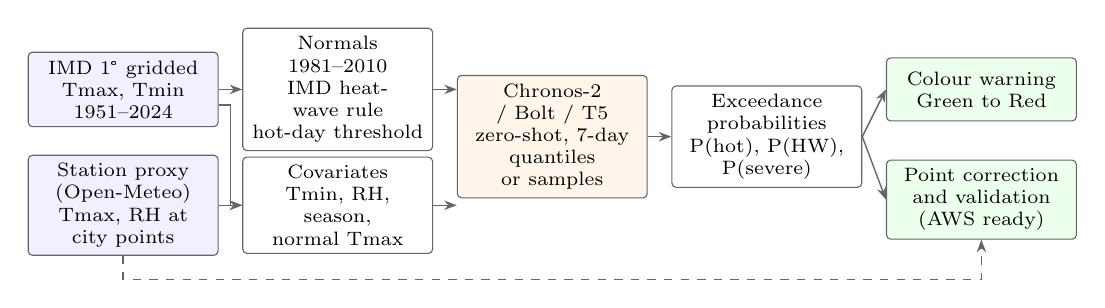
\begin{tikzpicture}[
  node distance=3.5mm and 3mm,
  box/.style={draw=black!60, rounded corners=1.5pt, align=center, font=\scriptsize, inner sep=3pt, minimum height=8mm, text width=22mm, fill=white},
  databox/.style={box, fill=blue!6},
  modelbox/.style={box, fill=orange!8},
  outbox/.style={box, fill=green!7},
  arr/.style={-{Stealth[length=1.6mm]}, draw=black!60, line width=0.5pt}
]
\node[databox] (imd) {IMD 1\textdegree{} gridded Tmax, Tmin\\1951--2024};
\node[databox, below=of imd] (om) {Station proxy (Open-Meteo)\\Tmax, RH at city points};
\node[box, right=of imd] (lab) {Normals 1981--2010\\IMD heatwave rule\\hot-day threshold};
\node[box, right=of om] (cov) {Covariates\\Tmin, RH, season,\\normal Tmax};
\node[modelbox, right=of lab, yshift=-6mm] (fm) {Chronos-2 / Bolt / T5\\zero-shot, 7-day\\quantiles or samples};
\node[box, right=of fm] (prob) {Exceedance\\probabilities\\P(hot), P(HW), P(severe)};
\node[outbox, right=of prob, yshift=6mm] (warn) {Colour warning\\Green to Red};
\node[outbox, right=of prob, yshift=-8mm] (loc) {Point correction\\and validation\\(AWS ready)};
\draw[arr] (imd) -- (lab);
\draw[arr] (om) -- (cov);
\draw[arr] (imd.east) ++(0,-2mm) -- ++(1.5mm,0) |- (cov.west);
\draw[arr] (lab.east) -- (fm.west |- lab.east);
\draw[arr] (cov.east) -- (fm.west |- cov.east);
\draw[arr] (fm) -- (prob);
\draw[arr] (prob.east) -- (warn.west);
\draw[arr] (prob.east) -- (loc.west);
\draw[arr, dashed] (om.south) -- ++(0,-3mm) -| (loc.south);
\end{tikzpicture}
}
\caption{HeatCast-FM pipeline. Gridded IMD data and point data feed labels and covariates. Chronos models produce 7-day quantile or sample forecasts, which become event probabilities, colour warnings and point-corrected forecasts.}
\label{fig:pipeline}
\end{figure*}

\subsection{Forecast setup}
A forecast is issued on every day from 1 March to 30 June. It uses the previous 512 days of data and predicts days 1 to 7. Years 1951-2014 are for training (baselines only), 2015-2018 for validation (warning thresholds, LSTM early stopping) and 2019-2024 for testing. Each season gives 122 issue dates per series, so the test set has \NTestForecasts{} forecasts and \NTestPairs{} forecast-observation pairs per model. Every model stores its forecast as 21 quantiles (levels 0.01, 0.05, 0.10, ..., 0.95, 0.99).

\subsection{Models}
\textbf{Persistence.} Tomorrow equals today, with the empirical distribution of training-period changes for each series, lead and month.

\textbf{Climatology.} The daily normal plus the distribution of anomalies seen within $\pm$15 days of the target date in 1985-2014.

\textbf{AR-anomaly.} An autoregressive model on daily anomalies. The order (up to 14) is chosen by AIC for each series. It gives Gaussian predictive intervals from the psi weights and a hot-season residual variance.

\textbf{Quantile-LSTM.} A two-layer LSTM \cite{hochreiter1997lstm} with 64 hidden units. Its inputs are 60 days of Tmax and Tmin anomalies with the sine and cosine of day of year. It outputs 7$\times$21 anomaly quantiles, is trained with the pinball loss on all series for 1951-2014, and uses early stopping on 2015-2018.

\textbf{Chronos-T5 (small, 46M).} This is the generative model. The context is mean-scaled and quantized into 4096 bins. A T5 encoder-decoder then samples the next token one day at a time, and we draw \TFiveSamples{} sample paths. Because of its cost it was run on the 7 focus regions only. We also rewrote the sampling loop so that the encoder runs once per series instead of once per sample.

\textbf{Chronos-Bolt (small).} Encodes patches of the context and emits 9 quantiles (0.1-0.9) for all steps at once. We extend these to our 21 levels with exponential tails fitted to the outer quantiles.

\textbf{Chronos-2 (120M).} An encoder-only model with group attention that emits 21 quantiles. We test three input sets:
\begin{itemize}
\item Tmax only.
\item \emph{+cov}: past Tmin and the normal Tmax, plus sine and cosine of day of year, where the normal and season terms are also given for the 7 target days as known future covariates.
\item \emph{+cov+RH}: the same with past relative humidity from the station proxy (focus regions only).
\end{itemize}

None of the Chronos models were fine-tuned.

\subsection{From quantiles to warnings}
For quantiles $q_1<\dots<q_{21}$ at levels $\tau_k$ we build a CDF $\hat F$ by linear interpolation. Beyond the outermost quantiles we use exponential tails matched to the two outermost quantiles on each side. The event probability is then $p=1-\hat F(\theta)$, where $\theta$ is the day's threshold for the hot-day, heatwave or severe event. For Chronos-T5 we can also count the share of sample paths above $\theta$. Both give almost the same result (Section~\ref{sec:results}).

The warning level for each target day is:
\begin{itemize}
\item \textbf{Yellow} (heat watch) if $p_{\text{hot}}\ge t_w$
\item \textbf{Orange} (heatwave alert) if $p_{\text{HW}}\ge t_a$
\item \textbf{Red} if $p_{\text{SEV}}\ge 0.5$
\end{itemize}
$t_w$ and $t_a$ maximise the critical success index (CSI) on 2015-2018 for leads 1-3. They are set separately for each model.

\subsection{Point validation and correction}
For each focus region and month we fit $T_{\text{point}}=a+b\,T_{\text{grid}}$ on 1990-2014 observations. The fitted map shifts and scales the grid forecast median. The spread is widened by the regression residual. Scores are then computed against the city-point Tmax, with IMD labels built from point normals.

\subsection{Humid heat}
For Mumbai, Ratnagiri and inland Pune we compute the NOAA heat index \cite{rothfusz1990} from point Tmax and minimum relative humidity. Minimum humidity approximates the humidity at the time of Tmax. We then count the March-June days in 1991-2024 on which the heat index reached the NOAA Danger level (39.4\,\textdegree C, 103\,\textdegree F) but the Tmax heatwave rule was not met.

\section{Results}\label{sec:results}
\subsection{Events in the study period}
Fig.~\ref{fig:thresholds} shows how the IMD rule plays out for three cities in 2019. At Mumbai the coastal threshold sits about 4.5\,\textdegree C above a normal of 35-36\,\textdegree C. At Pune the 40\,\textdegree C floor controls the threshold for most of the season. At Nagpur the threshold rises to the 45\,\textdegree C cap in May and early June, and the early June heat of 2019 crossed it. Table~\ref{tab:events} counts events over all \NSeries{} series. Hot days are common enough to verify at every region. IMD heatwave days are concentrated in Vidarbha, north Madhya Maharashtra and Marathwada, and most of them fall in 2019.

\begin{figure*}[t]
\centering
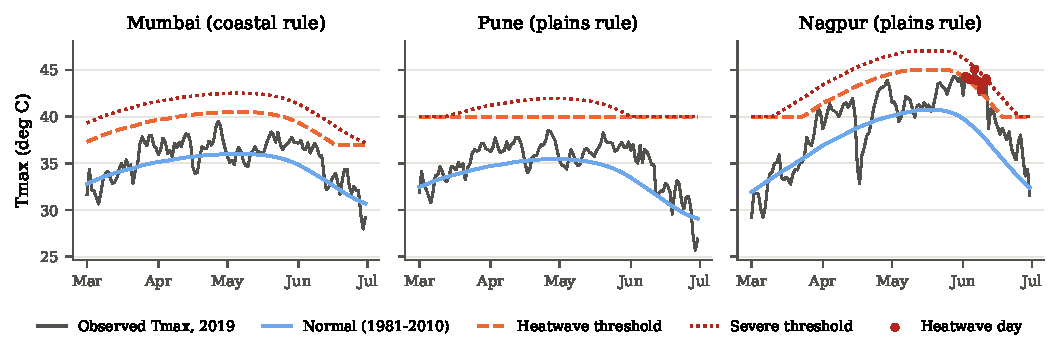
\includegraphics[width=\textwidth]{fig_thresholds.pdf}
\caption{Daily normal (1981-2010), IMD heatwave and severe thresholds, and observed IMD gridded Tmax for March-June 2019 at three focus regions. The same Tmax means different things under the coastal and plains rules.}
\label{fig:thresholds}
\end{figure*}

\subsection{Temperature forecast skill}
Table~\ref{tab:continuous} and Fig.~\ref{fig:lead} compare the models on all \NSeries{} series. Key points:
\begin{itemize}
\item \textbf{Best overall:} the quantile LSTM had the lowest CRPS (\CRPSQuantileLSTM\,\textdegree C) and the AR model was close behind (\CRPSARanomaly).
\item \textbf{Chronos, zero-shot:} Chronos-2+cov (\CRPSChronostwocov) and Chronos-2 (\CRPSChronostwo) were about 6\% worse than the LSTM. Chronos-Bolt was worse still (\CRPSChronosBolt).
\item \textbf{Versus simple references:} all three were well ahead of persistence (\CRPSPersistence) and climatology (\CRPSClimatology).
\item \textbf{Lead 1:} every model except climatology scored between 0.59 and 0.62\,\textdegree C.
\item \textbf{Leads 3 and 7:} the zero-shot models fell behind (Chronos-2+cov \CRPSChronostwocovLthree{} and \CRPSChronostwocovLseven{}, against \CRPSQuantileLSTMLthree{} and \CRPSQuantileLSTMLseven{} for the LSTM).
\end{itemize}

A block bootstrap over region-years puts the CRPS difference between \BootFM{} and \BootBL{} at \BootCRPS{} (95\% interval \BootCRPSlo{} to \BootCRPShi). This gap is small but significant, and it grows from \BootCRPSleadone{} at lead 1 to \BootCRPSleadseven{} at lead 7.

The Chronos models are overconfident. Their 80\% intervals held 75-78\% of observations, and Chronos-2+cov fell to about 72\% at longer leads (Fig.~\ref{fig:lead}, middle). The AR model was slightly too wide at short leads.

\begin{table*}[t]
\centering
\caption{Tmax forecast skill over all 43 series, test seasons 2019-2024, leads 1-7 pooled (deg C). CRPSS is relative to climatology. Cov80 is the share of observations inside the 10-90\% interval (target 0.80). Best value in bold.}
\label{tab:continuous}
\footnotesize
\setlength{\tabcolsep}{4pt}
\fitbox{%
\begin{tabular}{lrrrrrrrrr}
\toprule
Model & MAE & RMSE & CRPS & CRPSS & Cov80 & Width80 & CRPS d1 & CRPS d3 & CRPS d7 \\
\midrule
Chronos-2+cov & 1.375 & 1.861 & 0.988 & 0.173 & 0.75 & 3.89 & 0.616 & 0.967 & 1.179 \\
Chronos-2 & 1.379 & 1.876 & 0.989 & 0.172 & 0.77 & 4.19 & 0.614 & 0.962 & 1.197 \\
Chronos-Bolt & 1.422 & 1.965 & 1.019 & 0.147 & 0.78 & 4.32 & 0.603 & 0.974 & 1.274 \\
Quantile-LSTM & \textbf{1.299} & 1.807 & \textbf{0.935} & \textbf{0.217} & 0.78 & 3.85 & 0.606 & \textbf{0.921} & \textbf{1.099} \\
AR-anomaly & 1.315 & \textbf{1.767} & 0.943 & 0.211 & 0.82 & 4.32 & \textbf{0.593} & 0.932 & 1.112 \\
Persistence & 1.468 & 2.036 & 1.063 & 0.110 & 0.80 & 4.64 & 0.602 & 1.020 & 1.325 \\
Climatology & 1.690 & 2.234 & 1.194 & 0.000 & 0.77 & 5.00 & 1.188 & 1.193 & 1.197 \\
\bottomrule
\end{tabular}}
\end{table*}


\begin{figure*}[t]
\centering
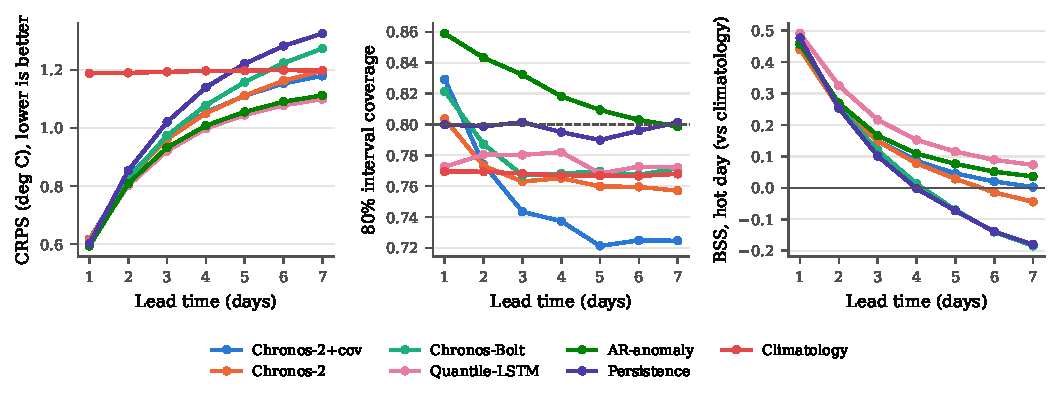
\includegraphics[width=\textwidth]{fig_skill_by_lead.pdf}
\caption{Skill against lead time over all 43 series, test seasons 2019-2024. Left: CRPS. Middle: share of observations inside the 80\% interval (dashed line is the target). Right: Brier skill score for the hot-day event, relative to climatology.}
\label{fig:lead}
\end{figure*}

\textbf{Effect of covariates.} On the 2015-2018 validation years, adding covariates lowered Chronos-2's CRPS from \ValCRPSChronostwo{} to \ValCRPSChronostwocov{}. That put it ahead of the AR model (\ValCRPSARanomaly) but still behind the LSTM (\ValCRPSQuantileLSTM). In the test years the pooled gain almost vanished, because it came in \CovBetterYears{} of \CovYearsTotal{} years and was offset by a large loss in 2023 (Section~\ref{sec:discussion}).

\subsection{Event probabilities}
Table~\ref{tab:eventskill} scores the event probabilities for leads 1-3.

\textbf{Hot days.} Every model beat climatology clearly on the hot-day event. The LSTM led (BSS \BSShotQuantileLSTM). Chronos-2+cov (\BSShotChronostwocov) was close to the AR model (\BSShotARanomaly).

\textbf{IMD heatwaves.} Discrimination was high for all models (AUC 0.96-0.98). Brier skill was much lower because the events are rare, and it varied widely: Chronos-Bolt (\BSShwChronosBolt) and persistence (\BSShwPersistence) were worse than climatology. For Bolt, the exponential tails we added beyond its 0.9 quantile likely give too much weight to extreme values.

\textbf{Calibration.} Fig.~\ref{fig:relroc} shows hot-day reliability and heatwave ROC curves. Chronos-2 slightly overforecasts at high probabilities. Chronos-2+cov and the LSTM stay closer to the diagonal.

\begin{table}[t]
\centering
\caption{Event probability skill over all 43 series, leads 1-3, test seasons (10,867 hot-day and 684 heatwave forecast-observation pairs out of 94,428). BSS is relative to climatology.}
\label{tab:eventskill}
\footnotesize
\setlength{\tabcolsep}{4pt}
\fitbox{%
\begin{tabular}{lrrrrrr}
\toprule
Model & BS hot & BSS hot & AUC hot & BS HW & BSS HW & AUC HW \\
\midrule
Chronos-2+cov & 0.0726 & 0.285 & 0.888 & 0.0062 & 0.112 & 0.964 \\
Chronos-2 & 0.0731 & 0.281 & 0.886 & 0.0065 & 0.079 & 0.974 \\
Chronos-Bolt & 0.0732 & 0.280 & 0.895 & 0.0085 & -0.208 & 0.982 \\
Quantile-LSTM & 0.0667 & \textbf{0.344} & 0.910 & 0.0057 & \textbf{0.183} & \textbf{0.983} \\
AR-anomaly & 0.0714 & 0.297 & 0.903 & 0.0060 & 0.142 & 0.976 \\
Persistence & 0.0735 & 0.277 & \textbf{0.912} & 0.0100 & -0.416 & 0.982 \\
\bottomrule
\end{tabular}}
\end{table}


\begin{figure*}[t]
\centering
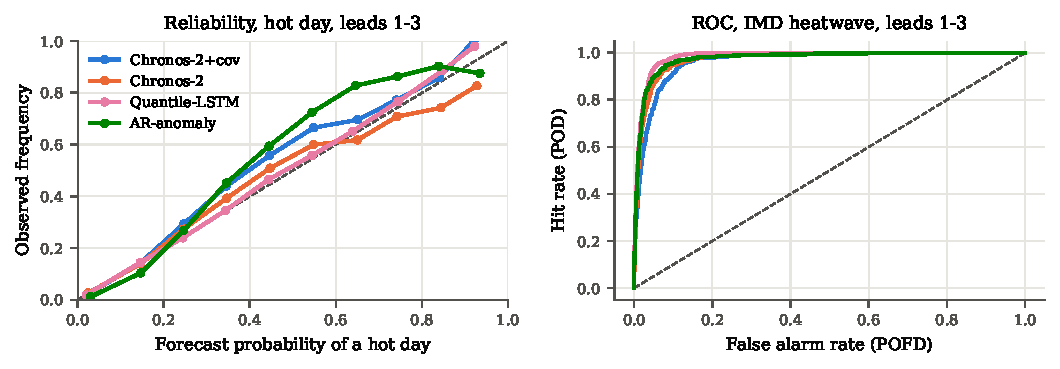
\includegraphics[width=0.72\textwidth]{fig_reliability_roc.pdf}
\caption{Left: reliability of hot-day probabilities. Right: ROC for IMD heatwave probabilities. Leads 1-3, all 43 series, test seasons.}
\label{fig:relroc}
\end{figure*}

\subsection{Focus regions, humidity and generative sampling}
Table~\ref{tab:focus} adds the three variants that were run only at the seven cities.

\begin{itemize}
\item \textbf{Humidity:} adding relative humidity to Chronos-2+cov lowered CRPS from \FocusCRPSChronostwocov{} to \FocusCRPSChronostwocovRH{}, the best Chronos result, though still behind the LSTM (\FocusCRPSQuantileLSTM).
\item \textbf{Generative sampling:} Chronos-T5, with \TFiveSamples{} sample paths, scored \FocusCRPSChronosTfive{}, slightly worse than persistence (\FocusCRPSPersistence).
\item \textbf{Samples versus quantiles:} for Chronos-T5, hot-day probabilities counted from the sample paths and read from the fitted quantiles agreed closely (correlation \TFiveCorr, Brier \TFiveBSsamp{} and \TFiveBSquant).
\end{itemize}

We also tried LoRA fine-tuning of Chronos-2+cov on the 1951-2014 series (rank 8, batch 32, context 512) but could not finish it on the laptop:
\begin{itemize}
\item \textbf{Apple GPU:} the first steps ran at about one per second, then slowed to about a minute per step.
\item \textbf{CPU:} about 68 seconds per step, so 300 steps would take over five hours.
\end{itemize}
The script is included for a GPU run.

\begin{table}[t]
\centering
\caption{Skill at the 7 focus regions (all models, test seasons). MAE and CRPS pool leads 1-7. Hot-day BSS and AUC use leads 1-3.}
\label{tab:focus}
\footnotesize
\setlength{\tabcolsep}{4pt}
\fitbox{%
\begin{tabular}{lrrrrrr}
\toprule
Model & MAE & CRPS & CRPSS & Cov80 & BSS hot & AUC hot \\
\midrule
Chronos-2+cov & 1.280 & 0.921 & 0.175 & 0.76 & 0.290 & 0.872 \\
Chronos-2+cov+RH & 1.256 & 0.907 & 0.188 & 0.76 & 0.301 & 0.878 \\
Chronos-2 & 1.278 & 0.921 & 0.175 & 0.78 & 0.295 & 0.873 \\
Chronos-Bolt & 1.329 & 0.957 & 0.143 & 0.79 & 0.294 & 0.881 \\
Chronos-T5 & 1.384 & 1.016 & 0.090 & 0.68 & 0.268 & 0.866 \\
Quantile-LSTM & \textbf{1.217} & \textbf{0.879} & 0.212 & 0.79 & \textbf{0.346} & 0.895 \\
AR-anomaly & 1.241 & 0.888 & 0.204 & 0.81 & 0.302 & 0.888 \\
Persistence & 1.388 & 1.007 & 0.098 & 0.80 & 0.291 & 0.894 \\
Climatology & 1.581 & 1.116 & 0.000 & 0.76 & 0.000 & 0.585 \\
\bottomrule
\end{tabular}}
\end{table}


\subsection{Warnings}
Table~\ref{tab:warnings} scores the colour warnings at the focus regions, where every model is compared on the same forecasts.

\begin{itemize}
\item \textbf{Yellow (hot-day watch):} CSI 0.36-0.41 for all models except climatology. The trained and zero-shot models were close.
\item \textbf{Orange (IMD heatwave alert):} Chronos-Bolt and Chronos-T5 had the highest CSI (\CSIorangeChronosBolt{} and \CSIorangeChronosTfive). They caught about 70\% of heatwave days at a false alarm ratio near 0.65. The LSTM had a lower FAR but missed most events. Its threshold, tuned on 2015-2018, was higher than the others (0.35).
\item \textbf{Across all 43 series:} Orange CSI was \AllCSIorangeChronosBolt{} for Bolt, \AllCSIorangeChronostwo{} for Chronos-2, \AllCSIorangeARanomaly{} for AR and \AllCSIorangeQuantileLSTM{} for the LSTM.
\item \textbf{Red:} with only \NSevPairs{} severe forecast-observation pairs in the test period, the Red level cannot be assessed.
\end{itemize}

\begin{table*}[t]
\centering
\caption{Warning verification at the 7 focus regions, leads 1-3, test seasons. Thresholds $t_w$ and $t_a$ were tuned for best CSI on 2015-2018. Yellow is checked against hot days, Orange against IMD heatwave days.}
\label{tab:warnings}
\footnotesize
\setlength{\tabcolsep}{4pt}
\fitbox{%
\begin{tabular}{lrrrrrrrr}
\toprule
Model & $t_w$ & POD & FAR & CSI & $t_a$ & POD & FAR & CSI \\
\midrule
Chronos-2+cov & 0.30 & 0.56 & 0.46 & 0.38 & 0.25 & 0.20 & 0.60 & 0.15 \\
Chronos-2+cov+RH & 0.25 & 0.67 & 0.51 & 0.39 & 0.25 & 0.32 & 0.64 & 0.21 \\
Chronos-2 & 0.25 & 0.66 & 0.52 & 0.39 & 0.20 & 0.66 & 0.68 & 0.27 \\
Chronos-Bolt & 0.30 & 0.70 & 0.52 & 0.40 & 0.40 & 0.69 & 0.65 & 0.30 \\
Chronos-T5 & 0.20 & 0.75 & 0.59 & 0.36 & 0.35 & 0.71 & 0.66 & 0.30 \\
Quantile-LSTM & 0.25 & 0.72 & 0.53 & 0.40 & 0.35 & 0.27 & 0.57 & 0.20 \\
AR-anomaly & 0.25 & 0.64 & 0.49 & 0.40 & 0.20 & 0.46 & 0.62 & 0.26 \\
Persistence & 0.45 & 0.64 & 0.46 & 0.41 & 0.60 & 0.36 & 0.49 & 0.27 \\
Climatology & 0.10 & 0.64 & 0.83 & 0.16 & 0.10 & 0.11 & 0.94 & 0.04 \\
\bottomrule
\end{tabular}}
\end{table*}


\subsection{Decision-support viewer}
The forecasts and warnings are served through a small Streamlit viewer (Fig.~\ref{fig:app}), in line with Objective 4 of the use case. A user picks a region, a model and an issue date. The viewer shows:
\begin{itemize}
\item the past three weeks of Tmax with the 7-day forecast fan, the IMD heatwave threshold and the hot-day threshold;
\item the overall warning colour for the week and the highest event probabilities;
\item a day-by-day table of median, 80\% range, threshold, event probabilities and warning level, with the observed Tmax when the date is in the past.
\end{itemize}
Dates in the backtest load from the saved forecasts. Any other date triggers a live Chronos-2 run, which takes a few seconds on the laptop. A static browser version with the same views for all saved forecasts is published with GitHub Pages at \url{https://aditya-ravi11.github.io/HeatCastFM/}, so the results can be explored without installing anything. Fig.~\ref{fig:app}(a) is the Nagpur forecast issued on 31 May 2019, one day before the heatwave: the viewer raised a Yellow heat watch with a 52\% chance of a hot day on 1 June, but gave the heatwave itself only 15\%, as discussed in the case studies. Fig.~\ref{fig:app}(b) is a quiet week at Mumbai in May 2024, where the coastal threshold of about 40.5\,\textdegree C was never in reach.

\begin{figure*}[t]
\centering
\begin{minipage}[t]{0.49\textwidth}\centering
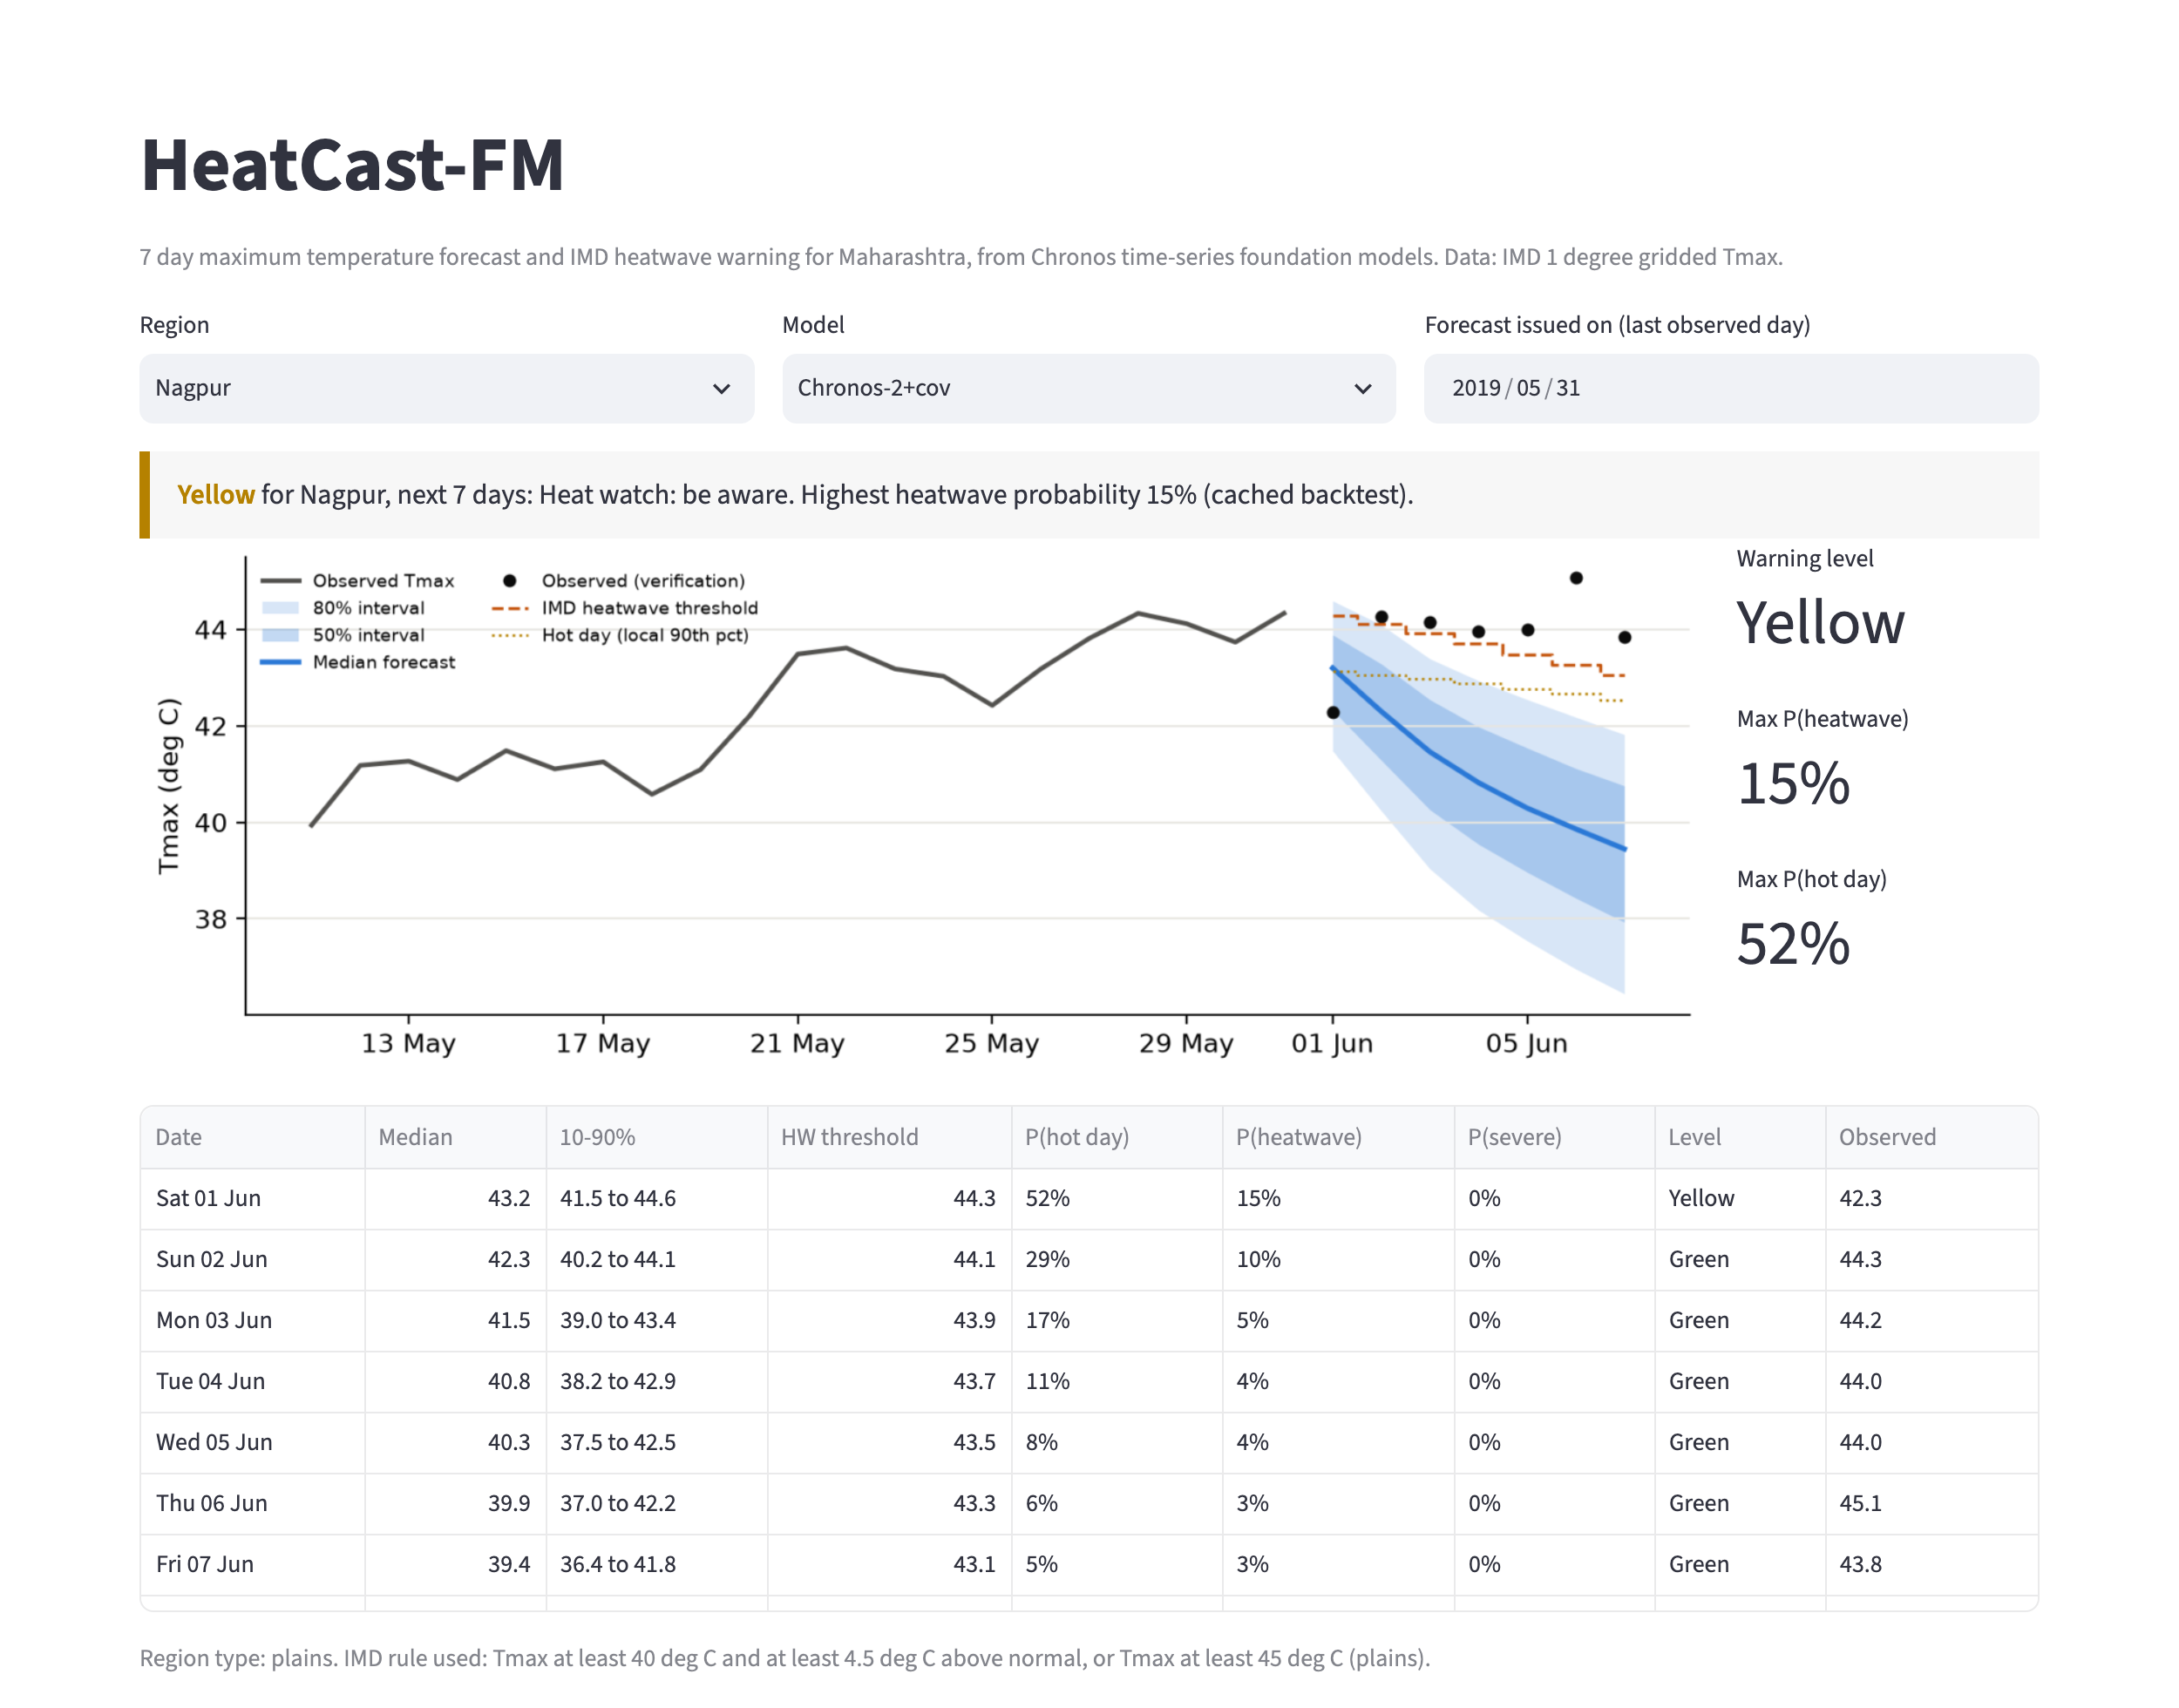
\includegraphics[width=\linewidth]{app/app_nagpur_2019.png}\\[1pt]
{\footnotesize (a) Nagpur, issued 31 May 2019: Yellow heat watch}
\end{minipage}\hfill
\begin{minipage}[t]{0.49\textwidth}\centering
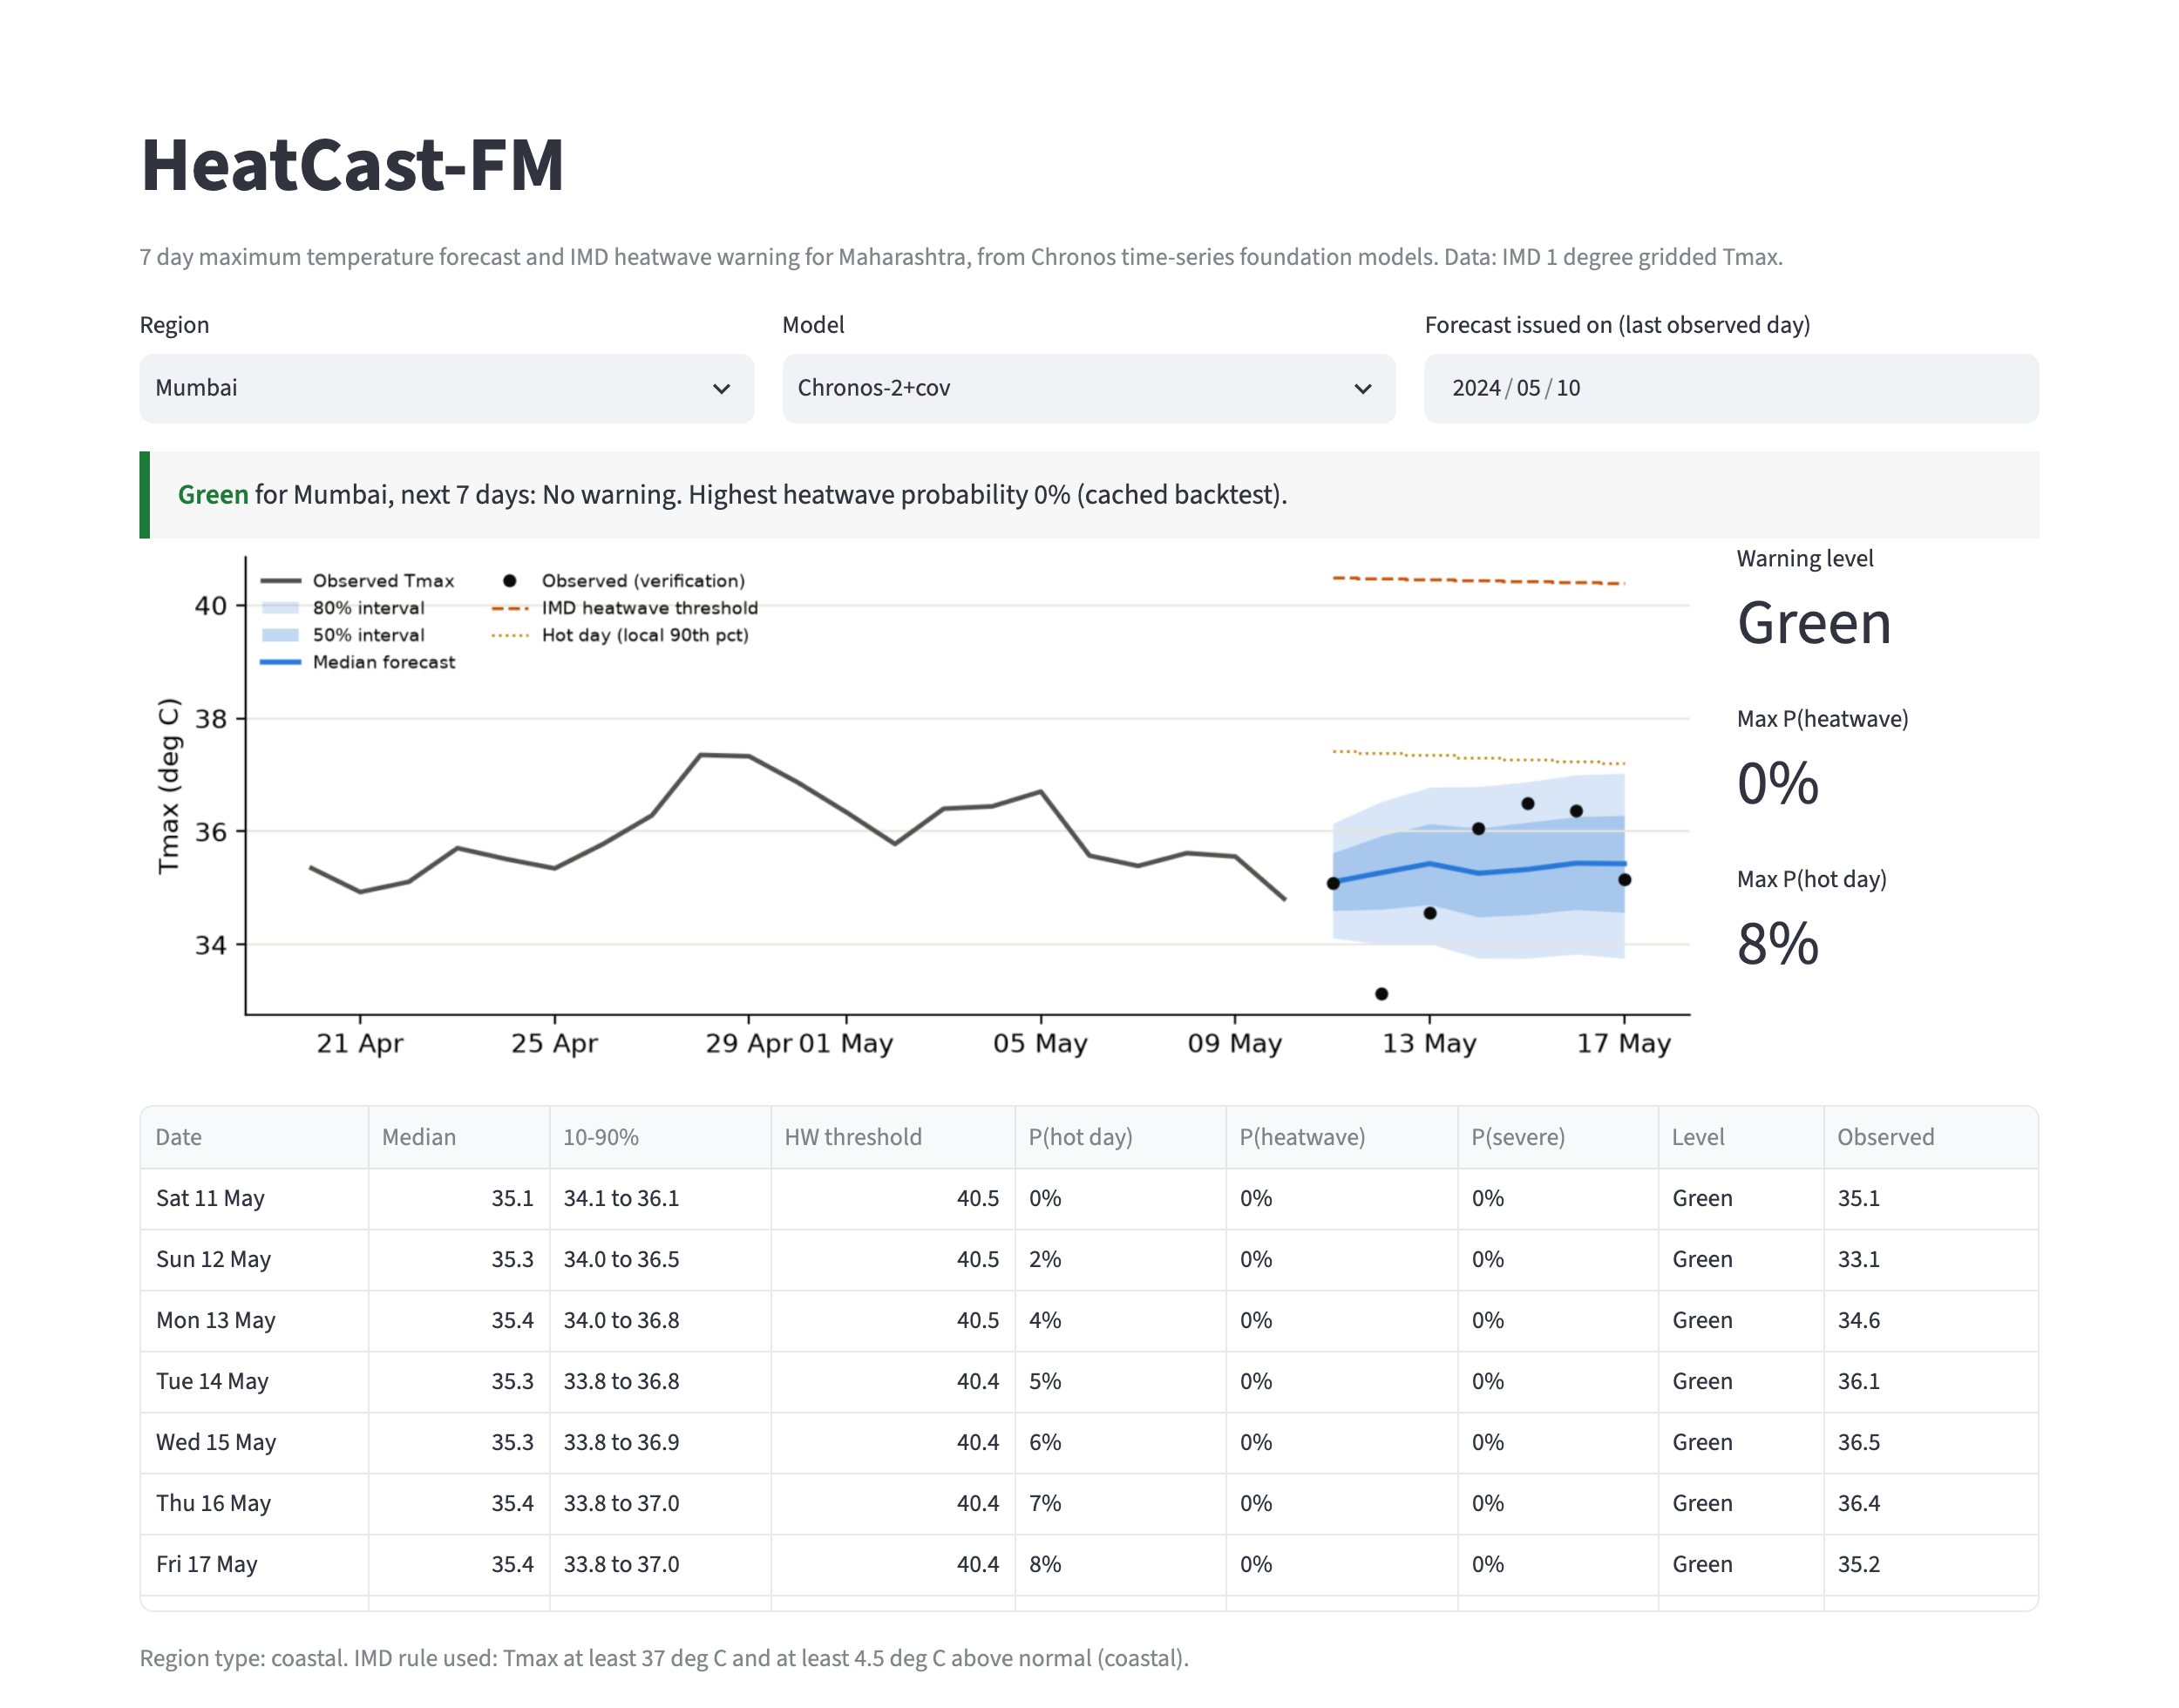
\includegraphics[width=\linewidth]{app/app_mumbai_2024.png}\\[1pt]
{\footnotesize (b) Mumbai, issued 10 May 2024: Green}
\end{minipage}
\caption{HeatCast-FM viewer (Streamlit) showing Chronos-2+cov forecasts. Each view gives the forecast fan against the IMD heatwave threshold, the warning level and a day-by-day table of event probabilities with verifying observations.}
\label{fig:app}
\end{figure*}

\subsection{Case studies}
Fig.~\ref{fig:cases} shows forecasts issued two days before the three longest heatwave spells at focus regions in the test years, all from late May and early June 2019. In each case both Chronos-2+cov and the AR model expected the heat to ease within the week. Instead it held at or above the threshold. At Jalgaon and Nagpur the 80\% bands still reached the threshold on the first days, so the heatwave probabilities were not zero even though the median was too low. At Chandrapur only the AR band did.

\begin{figure*}[t]
\centering
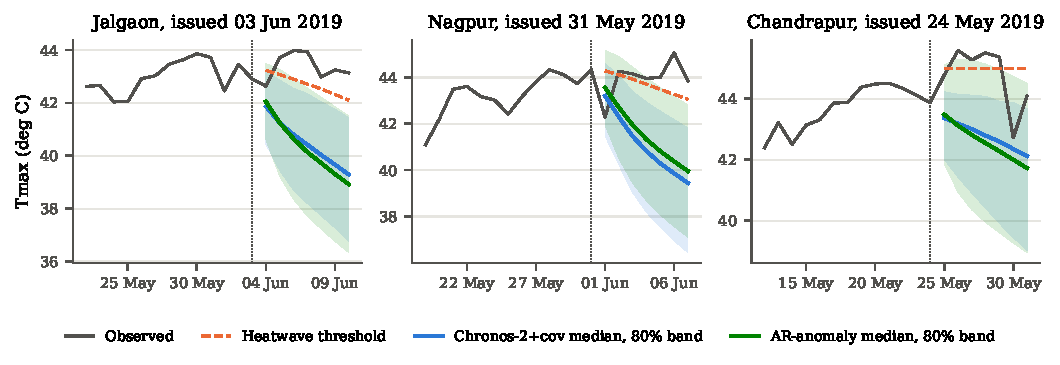
\includegraphics[width=\textwidth]{fig_cases.pdf}
\caption{Forecasts issued two days before the three longest heatwave spells at focus regions in 2019. Lines show the median, shading the 80\% band. The dashed orange line is the IMD heatwave threshold for each target day.}
\label{fig:cases}
\end{figure*}

\subsection{Point validation}
Table~\ref{tab:localization} checks Chronos-2+cov against city-point Tmax.

\textbf{Raw grid forecasts.} The raw forecasts had a mean point MAE of \LocMAEraw\,\textdegree C for leads 1-3, much larger than their error against the grid itself. The coastal cities and Sambhajinagar had the largest gaps, because the grid cell and the point differ by 1.9-2.6\,\textdegree C on average.

\textbf{After correction.} The monthly linear correction brought the mean point MAE down to \LocMAEcor\,\textdegree C and CRPS from \LocCRPSraw{} to \LocCRPScor. The correction helped most at Mumbai and Ratnagiri. It made results slightly worse at Chandrapur and Jalgaon, where the grid and the point already agreed well.

\begin{table*}[t]
\centering
\caption{Grid forecasts (Chronos-2+cov) checked against city-point Tmax, leads 1-3, test seasons. $r$ and bias (point minus grid, deg C) are from 1990-2014 March-July observations. HW is the number of point-level IMD heatwave days.}
\label{tab:localization}
\footnotesize
\setlength{\tabcolsep}{4pt}
\fitbox{%
\begin{tabular}{lrrrrrrr}
\toprule
Region & $r$ & Bias & MAE grid & MAE corr. & CRPS grid & CRPS corr. & HW \\
\midrule
Chandrapur & 0.88 & -0.93 & 1.52 & 1.62 & 1.11 & 1.15 & 32 \\
Jalgaon & 0.87 & -0.48 & 1.41 & 1.60 & 1.02 & 1.13 & 26 \\
Mumbai & 0.69 & -2.64 & 3.04 & 1.38 & 2.50 & 0.98 & 15 \\
Nagpur & 0.88 & 0.38 & 1.67 & 1.54 & 1.20 & 1.11 & 32 \\
Pune & 0.80 & -0.02 & 1.74 & 1.47 & 1.35 & 1.05 & 6 \\
Ratnagiri & 0.70 & -1.91 & 2.30 & 1.20 & 1.80 & 0.87 & 12 \\
Sambhajinagar & 0.87 & -2.17 & 2.31 & 1.31 & 1.73 & 0.93 & 6 \\
\bottomrule
\end{tabular}}
\end{table*}


\subsection{Humid heat at the coast}
Fig.~\ref{fig:humid} compares IMD Tmax-rule heatwave days with days when the heat index passed the NOAA Danger level (39.4\,\textdegree C) without a Tmax heatwave.

\begin{itemize}
\item \textbf{Mumbai:} \HumidMumbai{} such humid heat days in 1991-2024, against \TmaxhwMumbai{} Tmax-rule days.
\item \textbf{Ratnagiri:} \HumidRatnagiri{} humid heat days, against \TmaxhwRatnagiri{} Tmax-rule days.
\item \textbf{Pune (inland):} only \HumidPune{} humid heat days.
\end{itemize}

\begin{figure*}[t]
\centering
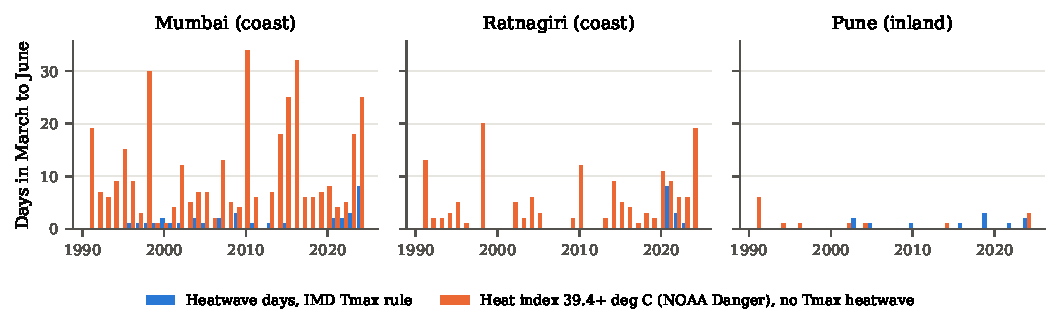
\includegraphics[width=\textwidth]{fig_humid_heat.pdf}
\caption{March-June days per year at two coastal cities and inland Pune (station proxy). Blue: IMD Tmax-rule heatwave days. Orange: days with heat index at or above 39.4\,\textdegree C (NOAA Danger) that the Tmax rule did not flag.}
\label{fig:humid}
\end{figure*}


\section{Discussion}\label{sec:discussion}
\textbf{What the foundation models do well.} The Chronos models were never shown Indian temperature data, yet Chronos-2 and Chronos-Bolt beat persistence and climatology on CRPS pooled over leads 1-7 (Chronos-T5 did not beat persistence at the focus regions). They also give usable probabilities: the hot-day reliability curves for Chronos-2 and Chronos-2+cov lie close to the diagonal, and their heatwave ROC areas are above 0.96. For an agency office that has to cover many districts with little data engineering, this is the main practical result. A single pretrained model, fed only the recent temperature history, produces calibrated-enough 7-day probabilities anywhere on the grid without a training step.

\textbf{Where they fall short.} Models trained on 64 years of local data remain better. The quantile LSTM and the AR model lead on CRPS, hot-day BSS and interval coverage. The gap is small at lead 1 and grows with lead time. The case studies in Fig.~\ref{fig:cases} show why. When a heatwave was already underway, every model, trained or not, forecast a return towards normal within a few days while the heat actually persisted. The trained baselines learn how fast anomalies at a given place and season decay. A zero-shot model has to infer that from 512 days of context, and it tends to relax too fast and with intervals that are too narrow (coverage \CovChronostwocov{} against the 0.80 target for Chronos-2+cov).

\textbf{Covariates.} Adding Tmin and the known seasonal normal to Chronos-2 improved the 2015-2018 validation CRPS clearly and helped in \CovBetterYears{} of the \CovYearsTotal{} test years. It was slightly worse in 2019 and clearly worse in 2023 (CRPS \CRPSChronostwocovYtwozerotwothree{} against \CRPSChronostwoYtwozerotwothree{}). The 2023 season had the second lowest mean Tmax anomaly of the six test years and several sharp drops in Tmax, and giving the model the normal as a future covariate seems to pull forecasts towards it during such cool spells. Relative humidity from the station proxy gave a further small gain at the focus regions (CRPS \FocusCRPSChronostwocovRH{} against \FocusCRPSChronostwocov{}). These results suggest covariates matter, but one validation period is not enough to choose them. A deployment would need a longer rolling check.

\textbf{Generative sampling.} Chronos-T5, the only model that generates sample paths token by token, was the weakest Chronos variant on continuous scores at the focus regions and by far the slowest (about \SpeedChronosTfive{} forecasts per second on the laptop, against about \SpeedChronostwo{} for Chronos-2). With only \TFiveSamples{} paths its probabilities are coarse. The share of paths above a threshold and the probability read from the fitted quantiles were almost the same (correlation \TFiveCorr{}), so sample paths add nothing that quantiles do not already give for this task. Its heatwave alerts tied with Chronos-Bolt for the best CSI at the focus regions, but that rests on 105 events and should be read with care.

\textbf{Limits of the grid.} The 1\textdegree{} IMD grid averages station values over about 100\,km, which lowers peaks. That is why the Mumbai and Pune cells never met the IMD rule in 2019-2024, while the point series met it on \LocPointHW{} region-days in the same seasons. Station rules applied to gridded data underestimate heatwave frequency. IMD also asks for the criteria to hold at two stations for two consecutive days. A single cell cannot test the first part; the 2-day variant in Table~\ref{tab:events} shows the second. Severe heatwaves were too rare on the grid (\NSevTest{} days in the test period) to verify the Red level at all.

\textbf{Station proxy.} Open-Meteo point data come from ERA5 reanalysis, not from a thermometer at the site. At Mumbai the proxy runs 2.6\,\textdegree C cooler than the grid cell on average, likely because the reanalysis cell at the coast includes sea surface. The point correction is therefore a correction to another model, and the results in Table~\ref{tab:localization} should be repeated once the use case's IoT weather stations are running. The loader and QC code for that are already in place.

\textbf{Humid heat.} The Tmax-only rule flagged \TmaxhwMumbai{} heatwave days at Mumbai in 1991-2024. Over the same seasons the heat index passed the NOAA Danger level on \HumidMumbai{} other days, about \HumidPerYearMumbai{} a year, against \HumidPerYearPune{} a year at inland Pune. This supports IMD's stated plan to fold humidity and warm nights into its criteria \cite{imd2026criteria}. With minimum humidity as the proxy for humidity at the time of Tmax, the heat index never reached IMD's experimental Orange band ($\ge$46\,\textdegree C). The highest value was \HImaxMumbai\,\textdegree C at Mumbai. So these counts depend on which humidity value and which threshold are used.


\section{Conclusion and Future Work}
HeatCast-FM shows that pretrained time-series foundation models can serve as the forecasting core of a regional heatwave warning system without any training on Indian data. Used zero-shot on IMD gridded Tmax, Chronos-2 with covariates gave 7-day probabilistic forecasts about 17\% better than climatology on CRPS. Its hot-day probabilities were reliable, and its heatwave ROC area was above 0.96. Models trained on 64 years of local data were still about 6\% better, with the gap growing with lead time. On this evidence, a foundation model is a good starting point for places or variables with short records. Where long local records exist, a well-built statistical or LSTM model remains hard to beat.

For the use case, the work delivers:
\begin{itemize}
\item a reproducible pipeline from IMD data to colour warnings;
\item a way to turn any quantile forecast into IMD rule probabilities for both coastal and plains stations;
\item a tested point correction that roughly halved the point error at Mumbai and Ratnagiri;
\item evidence that the Tmax-only rule misses many humid heat days on the Konkan coast;
\item a small viewer app that shows the 7-day forecast, event probabilities and warning level for any region and date.
\end{itemize}

Future work:
\begin{itemize}
\item replace the station proxy with the planned IoT weather stations and repeat the point validation;
\item complete the LoRA fine-tuning of Chronos-2 on a GPU;
\item calibrate the Chronos intervals on validation years, since they are too narrow;
\item test station data or finer temperature grids, where the official heatwave rule can be applied as intended;
\item add a humidity-aware warning level once IMD publishes its revised criteria.
\end{itemize}


\section*{Code and Data Availability}
All code, configuration, metric tables and figures are available at \url{https://github.com/aditya-ravi11/HeatCastFM}. The script \texttt{scripts/run\_all.sh} downloads the data and reproduces every table and figure. A browser version of the viewer is live at \url{https://aditya-ravi11.github.io/HeatCastFM/}, and the full viewer runs locally with \texttt{streamlit run app/streamlit\_app.py}.

\bibliographystyle{IEEEtran}
\bibliography{refs}

\end{document}
